\documentclass[a4paper]{article}

\newcommand{\worktype}{Лабораторная работа №3}
\newcommand{\workname}{Исследование бесконтактных датчиков приближения}
\newcommand{\teachername}{Быстров С.В.}
\newcommand{\studentname}{Овчинников П.А.}
\newcommand{\students}{368201, Зелепугин А.Ю. \\ 368606, Овчинников П.А. \\ 368725, Романова А.Д. \\ 285610, Чемякин А.А.}
\newcommand{\studystream}{СенСУ R22 бак 1.1}

\input{~/Документы/latex-boilerplates/settings.tex}

\addto\captionsrussian{\renewcommand{\figurename}{Рисунок}}
\captionsetup{labelsep=endash}

\begin{document}
\documentclass[a4paper]{article}

\newcommand{\worktype}{Домашняя работа №3}
\newcommand{\workname}{Плоский изгиб балки}
\newcommand{\teachername}{Моторин А.С.}
\newcommand{\studentname}{Овчинников П.А.}
\newcommand{\varnum}{10}
\newcommand{\groupnumber}{R3341}

\input{~/Documents/latex-boilerplates/settings.tex}

\begin{document}
\documentclass[a4paper]{article}

\newcommand{\worktype}{Домашняя работа №3}
\newcommand{\workname}{Плоский изгиб балки}
\newcommand{\teachername}{Моторин А.С.}
\newcommand{\studentname}{Овчинников П.А.}
\newcommand{\varnum}{10}
\newcommand{\groupnumber}{R3341}

\input{~/Documents/latex-boilerplates/settings.tex}

\begin{document}
\documentclass[a4paper]{article}

\newcommand{\worktype}{Домашняя работа №3}
\newcommand{\workname}{Плоский изгиб балки}
\newcommand{\teachername}{Моторин А.С.}
\newcommand{\studentname}{Овчинников П.А.}
\newcommand{\varnum}{10}
\newcommand{\groupnumber}{R3341}

\input{~/Documents/latex-boilerplates/settings.tex}

\begin{document}
\input{~/Documents/latex-boilerplates/titlepage.tex}

\end{document}

\end{document}

\end{document}

\textbf{Цель работы:} ознакомиться с устройством бесконтактных датчиков приближения, изучить принципы работы и схем включения.\\[0.5em]
\textbf{Порядок выполнения работы:}
\begin{enumerate}
    \item Получить набор исследуемых выключателей и определить их принадлежность к тому или иному типу по их серийным номерам с помощью сети Интернет. В набор входят следующие датчики: индуктивный, емкостный, оптический и магниточувствительный.
    \item По очереди для каждого датчика определить расстояние срабатывания и отпускания при использовании мишеней из различных материалов (4-5 шт.).
    \item Занести величину расстояний срабатывания и отпускания в таблицу. Повторить эксперимент несколько раз. Эксперимент проделать с разными мишенями. Для каждого датчика оформить свою таблицу.
    \item По полученным данным вычислить средние значения и разброс расстояний срабатывания и отпускания и занести полученные значения в таблицу. Для каждого датчика построить график зависимости выходного сигнала от расстояния до объекта, приняв состояние выходного сигнала «включено» за 1, а «выключено» — за 0. На одном графике поместить данные исследования датчика со всеми использованными материалами.
\end{enumerate}
\addsubsection{Основные технические характеристики исследуемых датчиков}
В работе исследуются четыре типа бесконтактных датчиков: индуктивный, ёмкостной, оптический и магнитный. В таблицах \ref{tab:csn}, \ref{tab:isn}, \ref{tab:ovn} и \ref{tab:mag} ниже приведены основные технические характеристики исследуемых датчиков.
\begin{table}[H]
    \caption{Основные технические характеристики ёмкостного датчика}
    \centering
    \begin{tabular}{|l|r|}
        \hline
        \multicolumn{2}{|c|}{\textbf{Ёмкостной датчик CSN E41A5-31P-10-LZ}} \\ \hline\hline
        \multicolumn{1}{|c|}{\textbf{Параметр}} & \multicolumn{1}{|c|}{\textbf{Значение}} \\ \hline
        Рабочее напряжение $U_{\text{раб}}$, В DC & 10\dots 30 \\ \hline
        Рабочий ток $I_{\text{раб}}$, мА & 400 \\ \hline
        Падение напряжения $U_d$ при $I_{\text{раб}}$, В & $\leqslant$2.5 \\ \hline
        Зазор (номинальный), мм & 10 \\ \hline
        Зазор (рабочий), мм & 0\dots 8 \\ \hline
        Максимальная частота переключения $F_{\text{макс}}$, Гц & 300 \\ \hline
        Гистерезис, \% & 3\dots 15 \\ \hline
        Диапазон температур, °C & -25\dots +75 \\ \hline
        Габариты кабеля подключения, мм$^2$ & 2$\times$0.34 \\ \hline
        Габариты (диаметр $\times$ шаг резьбы $\times$ длина), мм & М18$\times$1$\times$76 \\ \hline
    \end{tabular}
    \label{tab:csn}
\end{table}
\begin{table}[H]
    \caption{Основные технические характеристики индуктивного датчика}
    \centering
    \begin{tabular}{|l|r|}
        \hline
        \multicolumn{2}{|c|}{\textbf{Индуктивный датчик ISN EF41A-31P-8-LZ}} \\ \hline\hline
        \multicolumn{1}{|c|}{\textbf{Параметр}} & \multicolumn{1}{|c|}{\textbf{Значение}} \\ \hline
        Рабочее напряжение $U_{\text{раб}}$, В DC & 10\dots 30 \\ \hline
        Максимальный рабочий ток $I_{\text{макс}}$, мА & 250 \\ \hline
        Максимальное падение напряжения $U_d$ при $I_{\text{макс}}$, В & 2.5 \\ \hline
        Зазор (номинальный), мм & 8 \\ \hline
        Зазор (рабочий), мм & 0\dots 6.4 \\ \hline
        Максимальная частота переключения $F_{\text{макс}}$, Гц & 300 \\ \hline
        Диапазон температур, °C & -25\dots +75 \\ \hline
        Габариты кабеля подключения, мм$^2$ & 2$\times$0.34 \\ \hline
        Габариты (диаметр $\times$ шаг резьбы $\times$ длина), мм & М18$\times$1$\times$85 \\ \hline
    \end{tabular}
    \label{tab:isn}
\end{table}
\begin{table}[H]
    \caption{Основные технические характеристики оптического датчика}
    \centering
    \begin{tabular}{|l|r|}
        \hline
        \multicolumn{2}{|c|}{\textbf{Оптический датчик OV A43A-31P-150-LZ}} \\ \hline\hline
        \multicolumn{1}{|c|}{\textbf{Параметр}} & \multicolumn{1}{|c|}{\textbf{Значение}} \\ \hline
        Рабочее напряжение $U_{\text{раб}}$, В DC & 10\dots 30 \\ \hline
        Максимальный рабочий ток $I_{\text{макс}}$, мА & 250 \\ \hline
        Максимальное падение напряжения $U_d$ при $I_{\text{макс}}$, В & 2.5 \\ \hline
        Дальность действия, мм & 150 \\ \hline
        Допустимая ёмкость нагрузки, мкФ & 0.02 \\ \hline
        Максимальная освещённость рабочей среды, лк & 6000 \\ \hline
        Максимальная задержка срабатывания, мс & 5 \\ \hline
        Собственный ток потребления $I_o$, мА & $\leqslant$25 \\ \hline
        Частота циклов оперирования $f$, Гц & 100 \\ \hline
        Спектр излучения & инфракрасный \\ \hline
        Диапазон температур, °C & -15\dots +65 \\ \hline
        Габариты кабеля подключения, мм$^2$ & 2$\times$0.34 \\ \hline
        Габариты (диаметр $\times$ шаг резьбы $\times$ длина), мм & М18$\times$1$\times$86 \\ \hline
    \end{tabular}
    \label{tab:ovn}
\end{table}
\begin{table}[H]
    \caption{Основные технические характеристики магнитного датчика}
    \centering
    \begin{tabular}{|l|r|}
        \hline
        \multicolumn{2}{|c|}{\textbf{Оптический датчик OV A43A-31P-150-LZ}} \\ \hline\hline
        \multicolumn{1}{|c|}{\textbf{Параметр}} & \multicolumn{1}{|c|}{\textbf{Значение}} \\ \hline
        Напряжение коммутации $U_{\text{раб}}$, В DC & 10\dots 30 \\ \hline
        Ток коммутации $I_{\text{раб}}$, мА & 10\dots 250 \\ \hline
        Мощность $P_{\text{макс}}$, Вт акт. / ВА инд. & 10 / 0.6 \\ \hline
        Максимальная частота переключения $F_{\text{макс}}$, Гц & 400 \\ \hline
        Диапазон температур, °C & -25\dots +75 \\ \hline
        Габариты кабеля подключения, мм$^2$ & 2$\times$0.12 \\ \hline
        Габариты (длина $\times$ ширина $\times$ высота), мм & 27$\times$12.5$\times$11.15 \\ \hline
    \end{tabular}
    \label{tab:mag}
\end{table}

\addsubsection{Схема экспериментальной установки}
\begin{figure}[H]
    \centering
    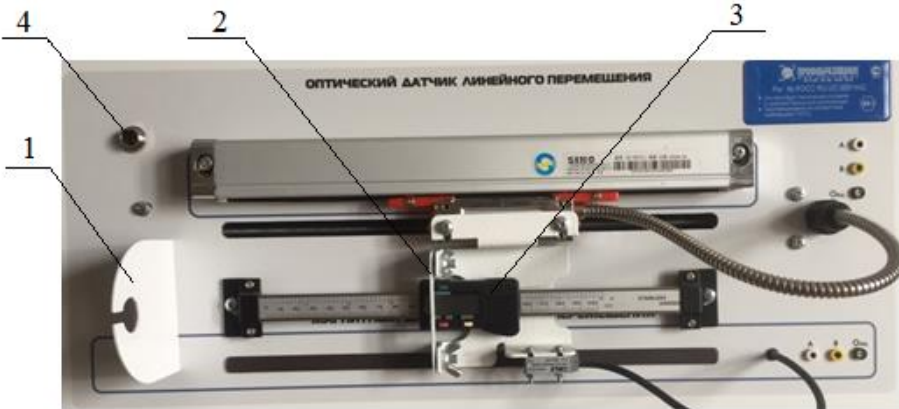
\includegraphics[width=0.5\textwidth]{scheme.png}
    \caption{Схема экспериментальной установки}
    \label{fig:exp}
\end{figure}
На рисунке \ref{fig:exp} представлена схема экспериментальной установки, где цифрами отмечены основные элементы установки:
\begin{enumerate}
    \item Неподвижная стойка, к которой крепится испытуемый датчик
    \item Передвижной механизм с креплением для мишени
    \item Измерительное устройство для замера величины перемещения мишени
    \item Разъем для подключения испытуемого датчика
\end{enumerate}
\newpage
\addsubsection{Характеристики используемых измерительных средств}
В рамках выполнения лабораторной работы использовалось только одно измерительное устройство — оптический датчик линейного перемещения. Оптический датчик прикреплён к передвижному механизму, которой двигается только в одной оси. Его характеристики приведены в таблице \ref{tab:odlp}.
\begin{table}[H]
    \centering
    \begin{tabular}{|l|r|}
        \hline
        \multicolumn{2}{|c|}{\textbf{Оптический датчик линейного перемещения}} \\ \hline\hline
        \multicolumn{1}{|c|}{\textbf{Параметр}} & \multicolumn{1}{|c|}{\textbf{Значение}} \\ \hline
        Диапазон измерений, мм & 0\dots 1000 \\ \hline
        Класс точности, мкм & $\pm$3 \\ \hline
    \end{tabular}
    \caption{Характеристики оптического датчика линейного перемещения}
    \label{tab:odlp}
\end{table}

\addsubsection{Результаты измерений и их обработка}
Результаты всех измерений, проведённых в ходе лабораторной работы, приведены в таблицах \ref{tab:csn_results}, \ref{tab:isn_results}, \ref{tab:ovn_results} и \ref{tab:mag_results}. В каждой таблице указаны расстояния срабатывания и отпускания для каждого из датчиков. Каждая таблица содержит 5 измерений для каждого материала мишени. Для ёмкостного, индуктивного и оптического датчиков использовались следующие материалы мишеней: стекло, металл, картон и пластик. Для магнитного датчика использовался только магнит.
\begin{table}[H]
    \caption{Расстояние срабатывания и отпускания ёмкостного датчика}
    \centering
    \begin{tabular}{|l|>{\raggedleft\arraybackslash}p{0.8cm}|>{\raggedleft\arraybackslash}p{0.8cm}|>{\raggedleft\arraybackslash}p{0.8cm}|>{\raggedleft\arraybackslash}p{0.8cm}|>{\raggedleft\arraybackslash}p{0.8cm}|>{\raggedleft\arraybackslash}p{0.8cm}|>{\raggedleft\arraybackslash}p{0.8cm}|>{\raggedleft\arraybackslash}p{0.8cm}|>{\raggedleft\arraybackslash}p{0.8cm}|>{\raggedleft\arraybackslash}p{0.8cm}|}
        \hline
        \multirow{2}{6em}{\centering \textbf{Материал мишени}} & \multicolumn{5}{|c|}{\textbf{Расстояние срабатывания, мм}} & \multicolumn{5}{|c|}{\textbf{Расстояние отпускания, мм}} \\ \cline{2-11}
        & \centering 1 & \centering 2 & \centering 3 & \centering 4 & \centering 5 & \centering 1 & \centering 2 & \centering 3 & \centering 4 & \centering 5 \arraybackslash \\ \hline
        Стекло  & 1.98 & 2.00 & 1.99 & 2.01 & 2.00 & 5.99 & 6.00 & 6.00 & 6.02  & 6.00 \\ \hline
        Металл  & 6.00 & 6.01 & 6.02 & 6.01 & 6.00 & 9.97 & 9.98 & 9.99 & 10.00 & 10.00 \\ \hline
        Картон  & 1.99 & 2.00 & 1.98 & 2.01 & 2.00 & 2.50 & 2.51 & 2.50 & 2.52  & 2.50 \\ \hline
        Пластик & 1.50 & 1.52 & 1.50 & 1.52 & 1.50 & 4.00 & 3.98 & 4.00 & 3.99  & 4.01 \\ \hline
    \end{tabular}
    \label{tab:csn_results}
\end{table}
\begin{table}[H]
    \caption{Расстояние срабатывания и отпускания индуктивного датчика}
    \centering
    \begin{tabular}{|l|>{\centering\arraybackslash}p{0.8cm}|>{\centering\arraybackslash}p{0.8cm}|>{\centering\arraybackslash}p{0.8cm}|>{\centering\arraybackslash}p{0.8cm}|>{\centering\arraybackslash}p{0.8cm}|>{\centering\arraybackslash}p{0.8cm}|>{\centering\arraybackslash}p{0.8cm}|>{\centering\arraybackslash}p{0.8cm}|>{\centering\arraybackslash}p{0.8cm}|>{\centering\arraybackslash}p{0.8cm}|}
        \hline
        \multirow{2}{6em}{\centering \textbf{Материал мишени}} & \multicolumn{5}{|c|}{\textbf{Расстояние срабатывания, мм}} & \multicolumn{5}{|c|}{\textbf{Расстояние отпускания, мм}} \\ \cline{2-11}
        & 1 & 2 & 3 & 4 & 5 & 1 & 2 & 3 & 4 & 5 \\ \hline
        Стекло  & — & — & — & — & — & — & — & — & —  & — \\ \hline
        Металл  & 9.98 & 9.99 & 10.01 & 10.00 & 10.00 & 10.00 & 10.01 & 10.00 & 10.02 & 10.01 \\ \hline
        Картон  & — & — & — & — & — & — & — & — & —  & — \\ \hline
        Пластик & — & — & — & — & — & — & — & — & —  & — \\ \hline
    \end{tabular}
    \label{tab:isn_results}
\end{table}
\begin{table}[H]
    \caption{Расстояние срабатывания и отпускания оптического датчика}
    \centering
    \begin{tabular}{|l|>{\raggedleft\arraybackslash}p{0.8cm}|>{\raggedleft\arraybackslash}p{0.8cm}|>{\raggedleft\arraybackslash}p{0.8cm}|>{\raggedleft\arraybackslash}p{0.8cm}|>{\raggedleft\arraybackslash}p{0.8cm}|>{\raggedleft\arraybackslash}p{0.8cm}|>{\raggedleft\arraybackslash}p{0.8cm}|>{\raggedleft\arraybackslash}p{0.8cm}|>{\raggedleft\arraybackslash}p{0.8cm}|>{\raggedleft\arraybackslash}p{0.8cm}|}
        \hline
        \multirow{2}{6em}{\centering \textbf{Материал мишени}} & \multicolumn{5}{|c|}{\textbf{Расстояние срабатывания, мм}} & \multicolumn{5}{|c|}{\textbf{Расстояние отпускания, мм}} \\ \cline{2-11}
        & \centering 1 & \centering 2 & \centering 3 & \centering 4 & \centering 5 & \centering 1 & \centering 2 & \centering 3 & \centering 4 & \centering 5 \arraybackslash \\ \hline
        Стекло  & 163 & 164 & 164 & 164 & 163 & 174 & 174 & 174 & 175 & 174 \\ \hline
        Металл  & 470 & 471 & 470 & 470 & 470 & 471 & 472 & 472 & 473 & 472 \\ \hline
        Картон  & 164 & 165 & 164 & 164 & 164 & 176 & 175 & 176 & 176 & 176 \\ \hline
        Пластик & 182 & 182 & 180 & 180 & 181 & 190 & 190 & 191 & 190 & 191 \\ \hline
    \end{tabular}
    \label{tab:ovn_results}
\end{table}
\begin{table}[H]
    \caption{Расстояние срабатывания и отпускания магнитного датчика}
    \centering
    \begin{tabular}{|l|>{\centering\arraybackslash}p{0.8cm}|>{\centering\arraybackslash}p{0.8cm}|>{\centering\arraybackslash}p{0.8cm}|>{\centering\arraybackslash}p{0.8cm}|>{\centering\arraybackslash}p{0.8cm}|>{\centering\arraybackslash}p{0.8cm}|>{\centering\arraybackslash}p{0.8cm}|>{\centering\arraybackslash}p{0.8cm}|>{\centering\arraybackslash}p{0.8cm}|>{\centering\arraybackslash}p{0.8cm}|}
        \hline
        \multirow{2}{6em}{\centering \textbf{Материал мишени}} & \multicolumn{5}{|c|}{\textbf{Расстояние срабатывания, мм}} & \multicolumn{5}{|c|}{\textbf{Расстояние отпускания, мм}} \\ \cline{2-11}
        & 1 & 2 & 3 & 4 & 5 & 1 & 2 & 3 & 4 & 5 \\ \hline
        Стекло  & — & — & — & — & — & — & — & — & — & — \\ \hline
        Металл  & — & — & — & — & — & — & — & — & — & — \\ \hline
        Картон  & — & — & — & — & — & — & — & — & — & — \\ \hline
        Пластик & — & — & — & — & — & — & — & — & — & — \\ \hline
        Магнит  & 4.00 & 4.01 & 4.00 & 4.01 & 4.00 & 7.01 & 7.00 & 7.01 & 7.01 & 6.98 \\ \hline
    \end{tabular}
    \label{tab:mag_results}
\end{table}
В случае с магнитным датчиком ни одна из мишеней не была обнаружена, поэтому мы воспользовались магнитом одного из студентов, чтобы всё же выполнить измерения.
\newpage
Обработаем измерения в таблицах \ref{tab:csn_results}, \ref{tab:isn_results}, \ref{tab:ovn_results} и \ref{tab:mag_results}. Для каждого датчика вычислим среднее значение и разброс расстояний срабатывания и отпускания. Результаты вычислений приведены в таблицах \ref{tab:csn_avg}, \ref{tab:isn_avg}, \ref{tab:ovn_avg} и \ref{tab:mag_avg} ниже.
\begin{table}[H]
    \caption{Средние значения и разброс расстояний срабатывания и отпускания ёмкостного датчика}
    \centering
    \begin{tabular}{|l|>{\centering\arraybackslash}p{2.6cm}|>{\centering\arraybackslash}p{2.6cm}|>{\centering\arraybackslash}p{2.6cm}|>{\centering\arraybackslash}p{2.6cm}|}
        \hline
        \multirow{2}{6em}{\centering \textbf{Материал мишени}} & \multicolumn{2}{|c|}{\textbf{Расстояние срабатывания, мм}} & \multicolumn{2}{|c|}{\textbf{Расстояние отпускания, мм}} \\ \cline{2-5}
        & Среднее & Разброс & Среднее & Разброс \\ \hline
        Стекло  & 2.00 & 0.03 & 6.00 & 0.03 \\ \hline
        Металл  & 6.01 & 0.02 & 9.99 & 0.03 \\ \hline
        Картон  & 2.00 & 0.03 & 2.51 & 0.02 \\ \hline
        Пластик & 1.51 & 0.02 & 4.00 & 0.03 \\ \hline
    \end{tabular}
    \label{tab:csn_avg}
\end{table}
\begin{table}[H]
    \caption{Средние значения и разброс расстояний срабатывания и отпускания индуктивного датчика}
    \centering
    \begin{tabular}{|l|>{\centering\arraybackslash}p{2.6cm}|>{\centering\arraybackslash}p{2.6cm}|>{\centering\arraybackslash}p{2.6cm}|>{\centering\arraybackslash}p{2.6cm}|}
        \hline
        \multirow{2}{6em}{\centering \textbf{Материал мишени}} & \multicolumn{2}{|c|}{\textbf{Расстояние срабатывания, мм}} & \multicolumn{2}{|c|}{\textbf{Расстояние отпускания, мм}} \\ \cline{2-5}
        & Среднее & Разброс & Среднее & Разброс \\ \hline
        Стекло  & — & — & — & — \\ \hline
        Металл  & 10.00 & 0.03 & 10.01 & 0.02 \\ \hline
        Картон  & — & — & — & — \\ \hline
        Пластик & — & — & — & — \\ \hline
    \end{tabular}
    \label{tab:isn_avg}
\end{table}
\begin{table}[H]
    \caption{Средние значения и разброс расстояний срабатывания и отпускания оптического датчика}
    \centering
    \begin{tabular}{|l|>{\centering\arraybackslash}p{2.6cm}|>{\centering\arraybackslash}p{2.6cm}|>{\centering\arraybackslash}p{2.6cm}|>{\centering\arraybackslash}p{2.6cm}|}
        \hline
        \multirow{2}{6em}{\centering \textbf{Материал мишени}} & \multicolumn{2}{|c|}{\textbf{Расстояние срабатывания, мм}} & \multicolumn{2}{|c|}{\textbf{Расстояние отпускания, мм}} \\ \cline{2-5}
        & Среднее & Разброс & Среднее & Разброс \\ \hline
        Стекло  & 164 & 1 & 174 & 1 \\ \hline
        Металл  & 470 & 1 & 472 & 2 \\ \hline
        Картон  & 164 & 1 & 176 & 1 \\ \hline
        Пластик & 181 & 2 & 190 & 1 \\ \hline
    \end{tabular}
    \label{tab:ovn_avg}
\end{table}
\begin{table}[H]
    \caption{Средние значения и разброс расстояний срабатывания и отпускания магнитного датчика}
    \centering
    \begin{tabular}{|l|>{\centering\arraybackslash}p{2.6cm}|>{\centering\arraybackslash}p{2.6cm}|>{\centering\arraybackslash}p{2.6cm}|>{\centering\arraybackslash}p{2.6cm}|}
        \hline
        \multirow{2}{6em}{\centering \textbf{Материал мишени}} & \multicolumn{2}{|c|}{\textbf{Расстояние срабатывания, мм}} & \multicolumn{2}{|c|}{\textbf{Расстояние отпускания, мм}} \\ \cline{2-5}
        & Среднее & Разброс & Среднее & Разброс \\ \hline
        Стекло  & — & — & — & — \\ \hline
        Металл  & — & — & — & — \\ \hline
        Картон  & — & — & — & — \\ \hline
        Пластик & — & — & — & — \\ \hline
        Магнит  & 4.00 & 0.01 & 7.00 & 0.03 \\ \hline
    \end{tabular}
    \label{tab:mag_avg}
\end{table}
Выбросы в измерениях оптического датчика с металлической мишенью связаны с тем, что поверхность металла отражает свет, и датчик не может обнаружить мишень с достаточно близкого расстояния.

\addsubsection{Графики снятых характеристик}
\begin{figure}[H]
    \centering
    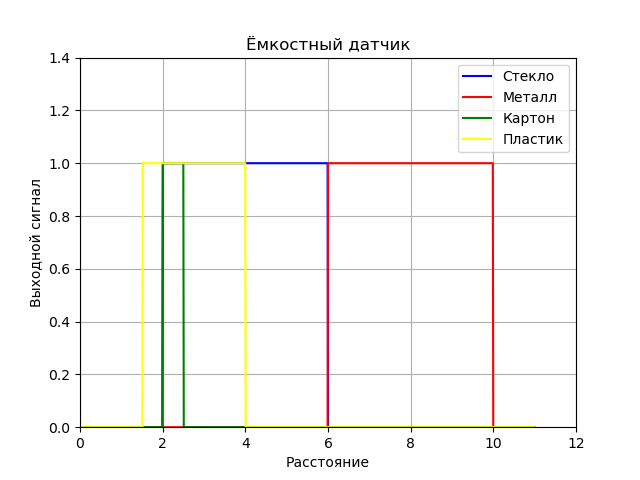
\includegraphics[width=0.7\textwidth]{plot_1.png}
    \caption{График снятых характеристик ёмкостного датчика}
    \label{fig:csn}
\end{figure}
\begin{figure}[H]
    \centering
    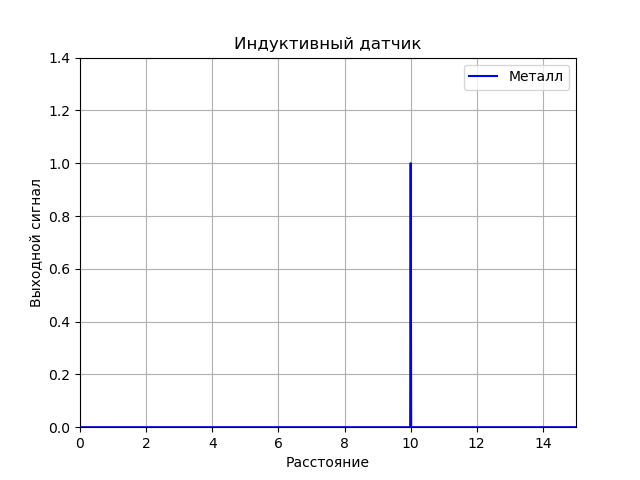
\includegraphics[width=0.7\textwidth]{plot_2.png}
    \caption{График снятых характеристик индуктивного датчика}
    \label{fig:isn}
\end{figure}
\begin{figure}[H]
    \centering
    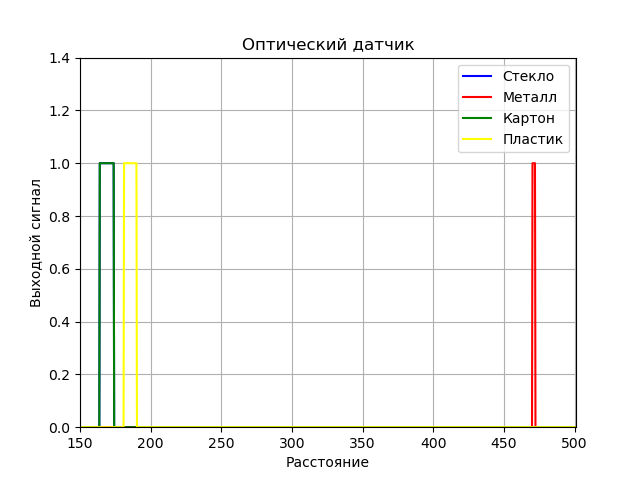
\includegraphics[width=0.7\textwidth]{plot_3.png}
    \caption{График снятых характеристик оптического датчика}
    \label{fig:ovn}
\end{figure}
\begin{figure}[H]
    \centering
    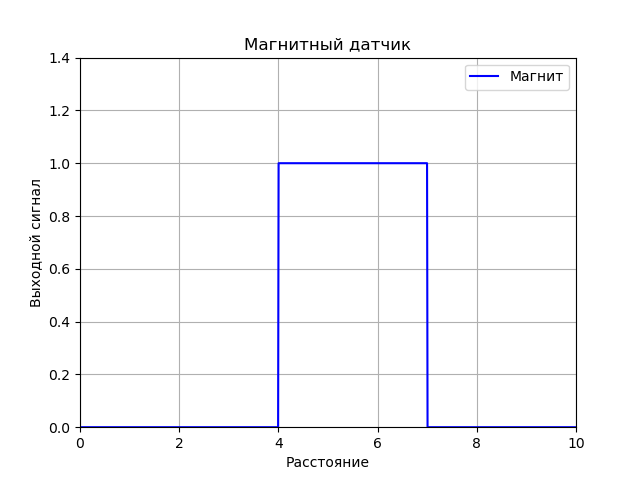
\includegraphics[width=0.7\textwidth]{plot_4.png}
    \caption{График снятых характеристик магнитного датчика}
    \label{fig:mag}
\end{figure}
\addsubsection{Выводы}
В ходе выполнения лабораторной работы исследованы четыре типа бесконтактных датчиков: индуктивный, ёмкостной, оптический и магнитный. Для каждого датчика получены средние значения и разброс расстояний срабатывания и отпускания и также определена зависимость выходного сигнала от расстояния до объекта. В результате эксперимента установлено, что индуктивный датчик распознаёт только мишени с достаточной электропроводностью, а магнитному датчику требует магнитное поле.\\[0.5em]
В ходе лабораторной работы закреплены теоретические знания о бесконтактных датчиках и их применении в различных областях, а также практические навыки работы с датчиками и обработки полученных данных.
\end{document}